\section{Phase II}
\label{sec:phase2}

Figure~\ref{fig:RxTx} shows the complete Block Diagram. For this second phase 2 blocks are added, Interleaver and error control. 

\subsection{Interleaver}

The \textbf{Interleaver} will shuffle the bit order, because errors tend to happen in bursts, this way the code correction/detection block is more efficient. Hence, the interleaver order is of importance, it must be after error control, otherwise it will be useless, and less obviously it must be before Modulation, because each modulated symbol is represents more than 1 bit, therefore an interleaver for the modulated symbols will have bit error bursts. For the simulation, this block should be more effective for Rayleigh because it has more bursts, compared to AWGN where it is just white noise. 

\subsection{Error Control}

For both error-control schemes the MATLAB processing chain is identical: the plain-text message is encoded, protected by the selected error control stage, interleaved, and modulated. After transmission through the channel, the signal is demodulated, de-interleaved, and decoded in reverse order, and the resulting bits are compared with the original data to compute the error statistics.

\subsubsection{Convolutional}

The convolutional coding uses 64 states and has a code rate $R = 1/3$, constraint length $K = 7$ and generator polinomial $G_0 = 133$, $G_1=171$ and $G_3 = 165$. 

\subsubsection{Hamming}

The other block-coding stage employed is the binary Hamming $(15,11)$ code. It maps every $k=11$ information bits into an $n=15-bit$ codeword, adding four parity bits according to the generator matrix, The code can correct any single-bit error and detect (but not correct) any double-bit error in each 15-bit word.

\subsubsection{Theoretical re-transmission probability}

For a $(15,11)$ Hamming code an ARQ is triggered if the decoder
detects \(\ge 2\) bit errors in the codeword. The probability is Equation \ref{eq:Pret}.

\begin{equation}
      P_{ret} \approx \begin{pmatrix}n \\ 1\end{pmatrix}p(1-p)^{n-1} \text{\cite{Work_TAC2025}}
      \label{eq:Pret}
\end{equation}

Where the it error probabilities are: 

\begin{equation}
      P_b^{\text{QPSK, Rayleigh}} = \frac{1}{2} \left( 1 - \sqrt{ \frac{E_b / N_0}{1 + E_b / N_0} } \right )
\end{equation}

\begin{equation}
      P_b^{\text{16QAM, Rayleigh}} = \frac{3}{4} \left( 1 - \sqrt{ \frac{ \frac{4}{5} \, E_b / N_0 }{ 1 + \frac{4}{5} \, E_b / N_0 } } \right )
\end{equation}


This yields Figure \ref{fig:Pret_Teo}.

\begin{figure}[H]
  \centering
  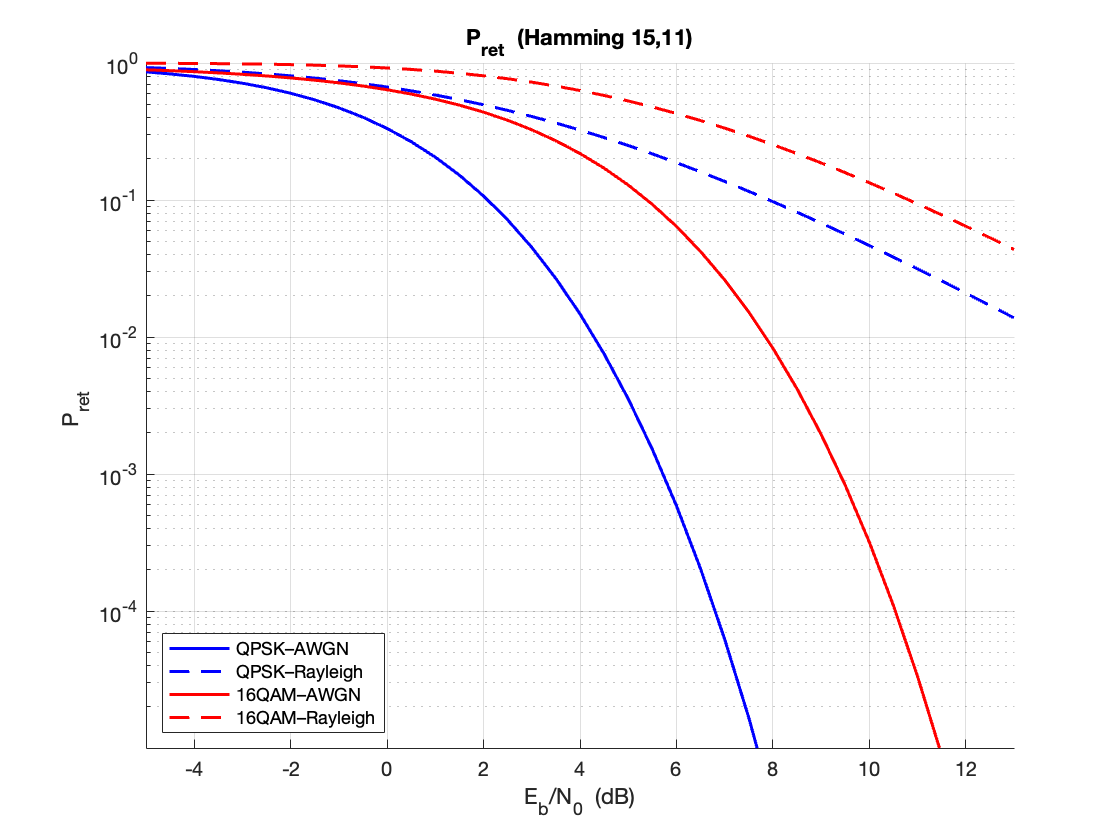
\includegraphics[width=0.7\linewidth]{Images/Pret_hamm.png}
  \caption{Theoretical retransmission probability.}
  \label{fig:Pret_Teo}
\end{figure}

\subsection{Simulation results}

It is important to note that as previously stated, for Huffman or ASCII encoding, the results should not change for the BER performance, hence only the Huffman encoded Bit stream was used. In order to maintain comparable graphs, all graphs are BER as a function of SNR. For this section since simulations took considerably longer, the number of bits sent returned again to 1 million.

First simulating only with the convolutional coding, Figure \ref{fig:Conv_BER}. This shows that BER quickly drops.

\begin{figure}[H]
  \centering
  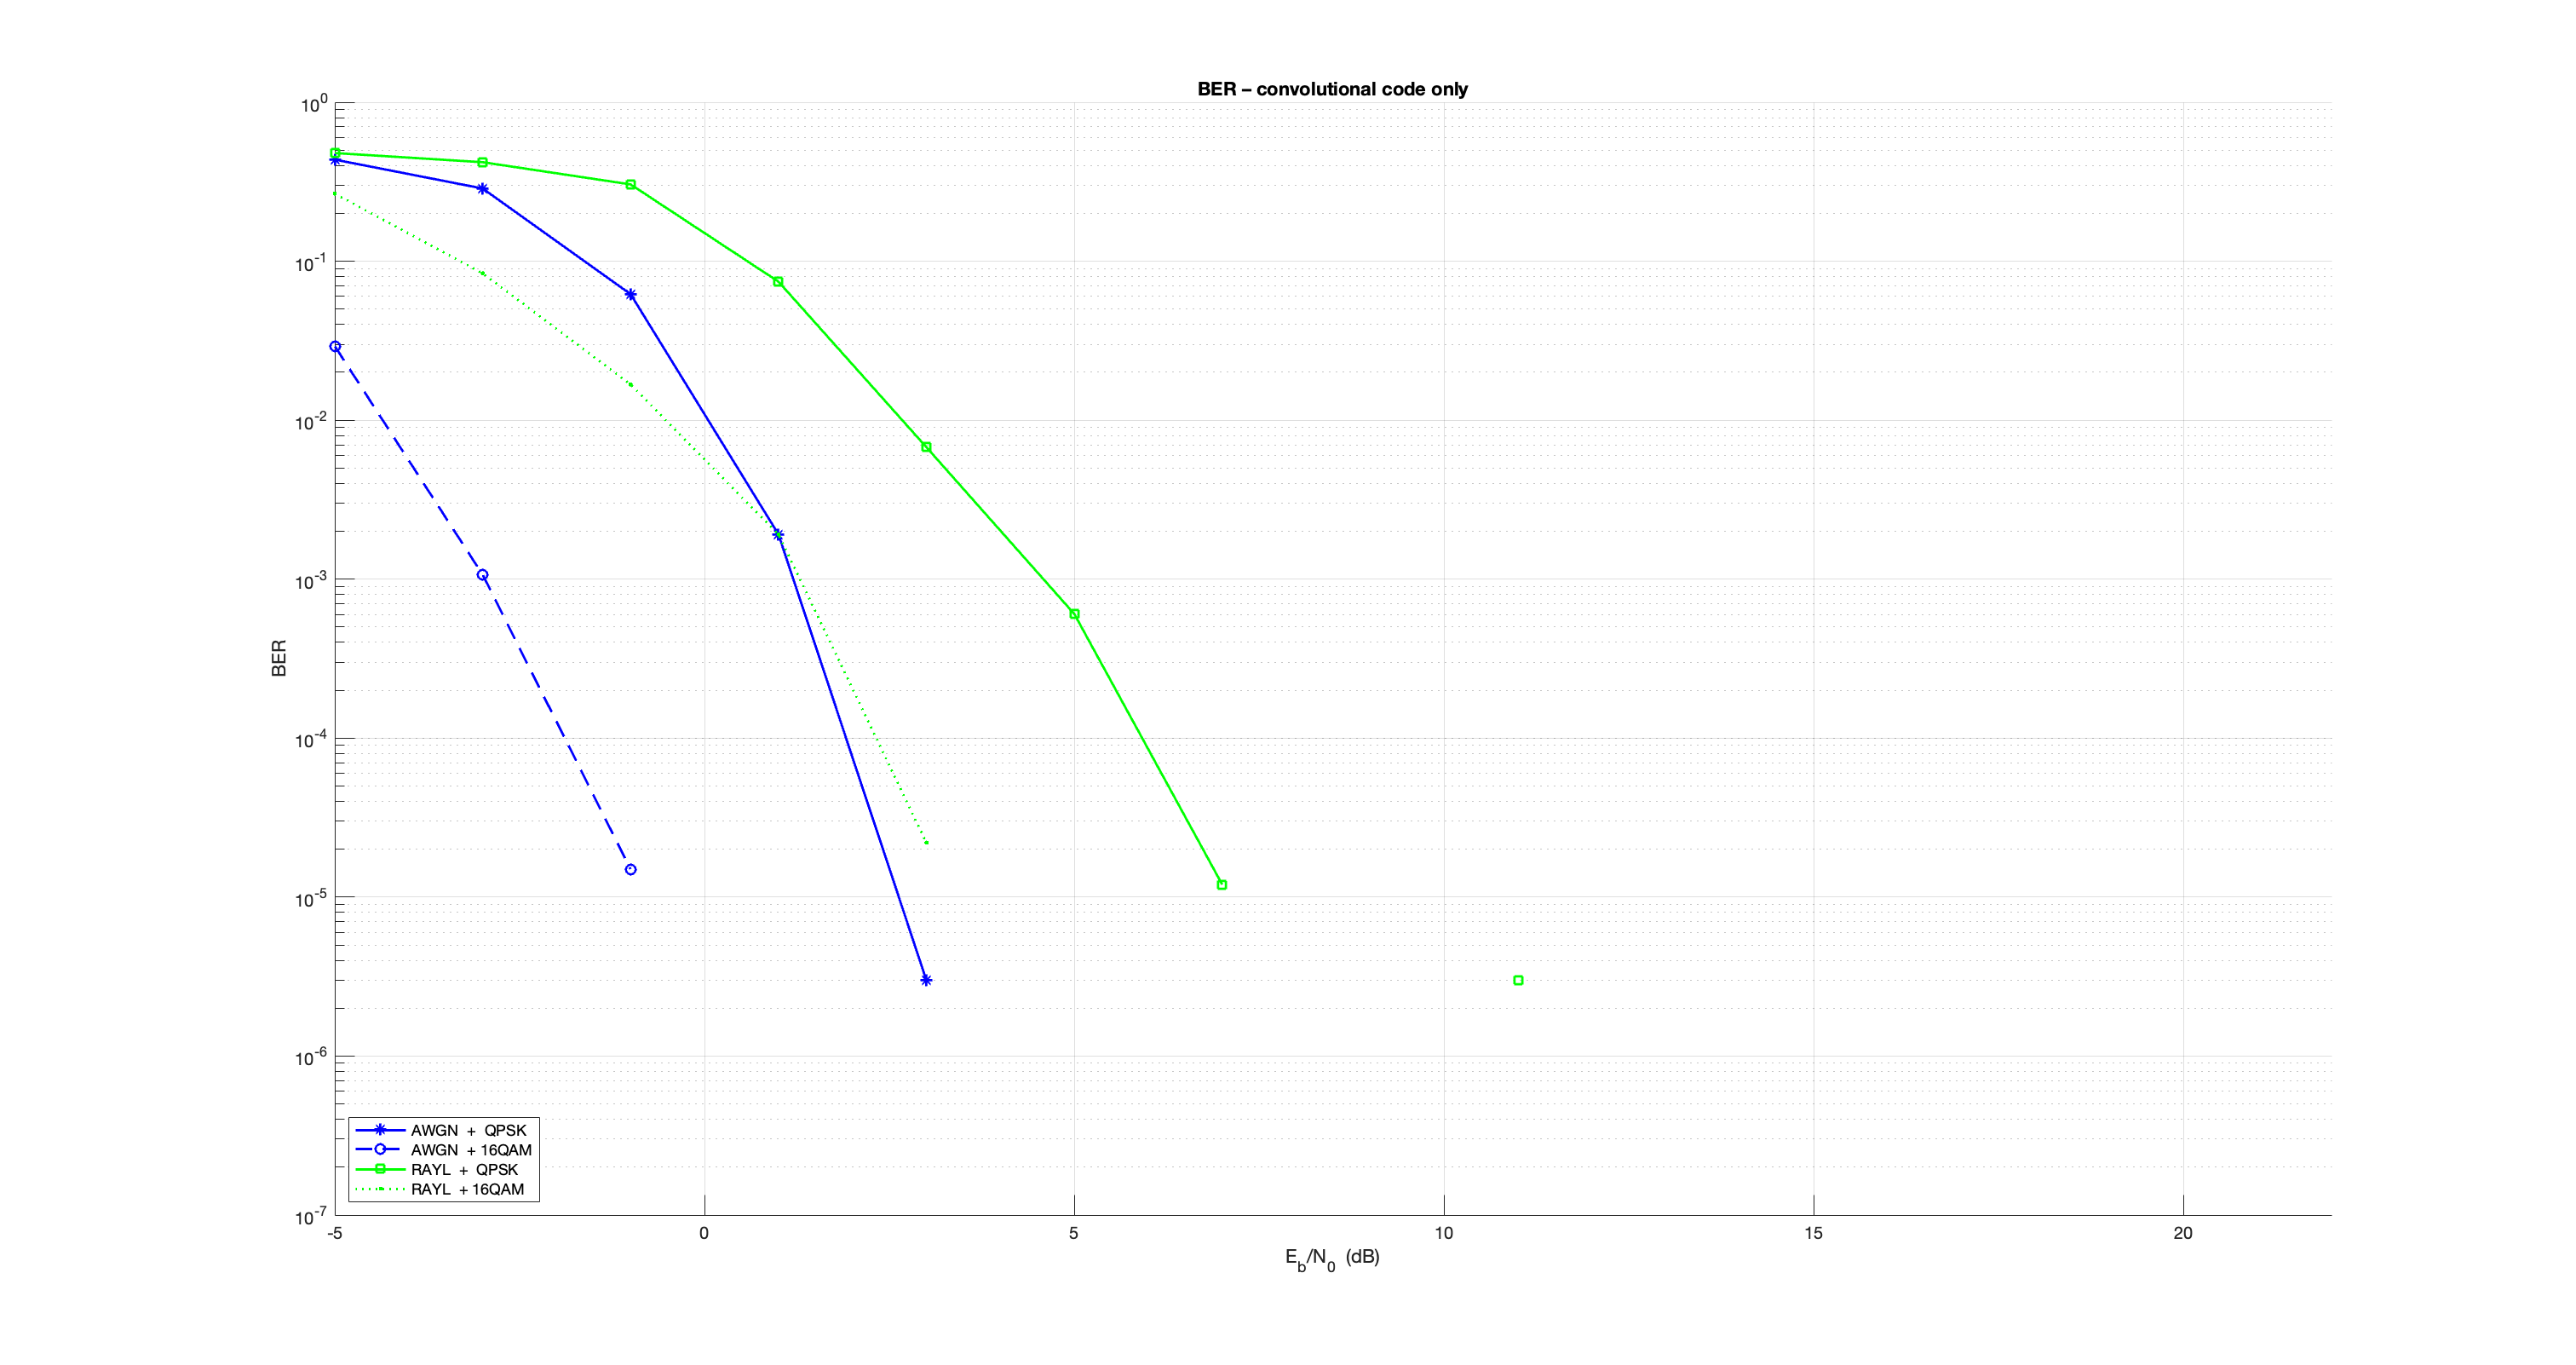
\includegraphics[width=0.7\linewidth]{Images/ConvCode.png}
  \caption{Convolutional  coding BER vs.\ $E_b/N_0$.}
  \label{fig:Conv_BER}
\end{figure}

After this the Hamming(15,11) was simulated, Figure \ref{fig:Hamm_BER}. This shows that BER does not drop as quickly.

The simulated retransmission probability was also calculated, Figure \ref{fig:Pret_sim}.

\begin{figure}[H]

    \centering
    \begin{subfigure}{0.45\textwidth}
        \includegraphics*[scale = 0.18]{Images/BlockCode.png}
        \caption{BER vs.\ $E_b/N_0$.}
        \label{fig:Hamm_BER}
    \end{subfigure}
    %\hfill
    \begin{subfigure}{0.45\textwidth}
        \includegraphics*[scale = 0.19]{Images/BlockCode.png}
        \caption{Retransmission Probability.}
        \label{fig:Pret_Sim}
    \end{subfigure}
    
    \caption{Hamming(15,11), performance metrics.}
    \label{fig:Hamm_performance}
\end{figure}


Finally with both methods, Figure \ref{fig:Both_BER}, showing the best performance over all.

\begin{figure}[H]

    \centering
    \begin{subfigure}{0.45\textwidth}
        \includegraphics*[scale = 0.18]{Images/BlockConvCode.png}
        \caption{BER vs.\ $E_b/N_0$.}
        \label{fig:Both_BER}
    \end{subfigure}
    %\hfill
    \begin{subfigure}{0.45\textwidth}
        \includegraphics*[scale = 0.19]{Images/BlockConvCode.png}
        \caption{Retransmission Probability.}
        \label{fig:Pret_Both_Sim}
    \end{subfigure}
    
    \caption{Hamming(15,11) + Convolutional, performance metrics.}
    \label{fig:Both_performance}
\end{figure}

When comparing to Figure \ref{fig:BER_SNR}, where there is no error correction nor detection there is a clear improvement for all cases, alone convolutional coding shows the best improvement, but by combining both methods the system is able to low BER in a noisy channel.